\section{Anexos}

\subsection{Manual de usuario}
\label{manual-usuario}
\subsubsection{Menú de Navegación}

El menú de navegación es una de las partes más necesarias de aclarar puesto que a través de él los usuarios pueden acceder a las diferentes secciones de la aplicación de manera sencilla e intuitiva. El menú está ubicado en la parte superior de la pantalla y contiene enlaces directos a las funcionalidades principales, como el inicio, Rutas de viaje, configuración de perfil y vista de proveedor. Además, el menú es responsivo, adaptándose a distintos tamaños de pantalla para garantizar una experiencia óptima tanto en computadoras como en dispositivos móviles.

 \vspace{2mm}
    \begin{minipage}{0.9\textwidth}
    \centering
    \captionof{figure}[{Barra de navegación.}]{Barra de navegación.}
    \label{ManualBarraNavegacion}
    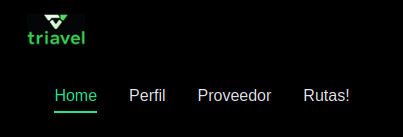
\includegraphics[width=0.7\textwidth]{Content/Images/ManualBarraNavegacion.png}
    \footnote{Nota. \textup{Fuente : Autores.}}
    \end{minipage}



La barra de busqueda permite a los usuarios encontrar rutas, destinos o proveedores de manera rápida y eficiente. Al escribir una palabra clave en la barra de búsqueda, el sistema sugiere resultados relevantes en tiempo real, facilitando la navegación y el acceso a la información deseada. Esta funcionalidad mejora significativamente la experiencia del usuario al reducir el tiempo necesario para localizar opciones específicas dentro de la aplicación.

     \vspace{2mm}
    \begin{minipage}{0.9\textwidth}
    \centering
    \captionof{figure}[{Barra de Busqueda.}]{Barra de Busqueda.}
    \label{ManualBarraNavegacion}
    
\includegraphics[width=0.7\textwidth]{Content/Images/ManualBarraBusqueda.png}
    \footnote{Nota. \textup{Fuente : Autores.}}
    \end{minipage}


    Los botones principales de busqueda para filtrar los Restaurantes, hoteles y demás sitios turísticos ayudan a filtrar los espacios para que aparezcan de acuerdo a las necesidades del usuario.

      \vspace{2mm}
    \begin{minipage}{0.9\textwidth}
    \centering
    \captionof{figure}[{Botones de busqueda.}]{Botones de busqueda.}
    \label{ManualBarraNavegacion}
    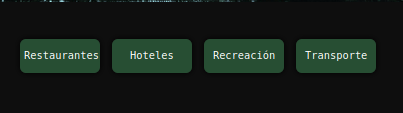
\includegraphics[width=0.7\textwidth]{Content/Images/ManualBotonesDeBusqueda.png}
    \footnote{Nota. \textup{Fuente : Autores.}}
    \end{minipage}

    Los botones de carrusel permiten el desplazamiento entre los diferentes elementos dispuestos entre carruseles, sean lugares, noticias o reseñas.

      \vspace{2mm}
    \begin{minipage}{0.9\textwidth}
    \centering
    \captionof{figure}[{Botones de busqueda.}]{Botones de busqueda.}
    \label{ManualBarraNavegacion}
    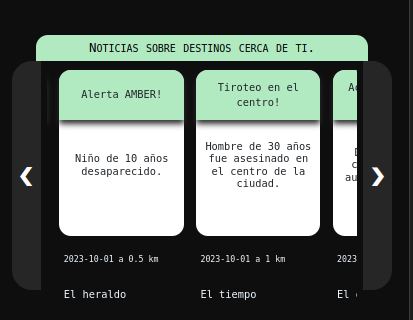
\includegraphics[width=0.7\textwidth]{Content/Images/ManualFlechasCarrusel.png}
    \footnote{Nota. \textup{Fuente : Autores.}}
    \end{minipage}


    \subsection{Criteriors de aceptación}
    
    1. Las funcionalidades del aplicativo  estar terminadas en un 90\% y probadas antes de final del primer año de producción.
    
    2. Pese a que se propone un margen de presupuesto destinado a riesgos, se espera que el desarrollo del proyecto no consuma la totalidad de este presupuesto, el criterio de aceptación entonces es que no consuma mas del 60\% del presupuesto destinado a riesgos.

    3. El aplicativo debe ser capaz de soportar un mínimo de 1000 usuarios concurrentes después del primer año de desarrollo sin degradar su rendimiento, garantizando una experiencia fluida y eficiente para todos los usuarios.

    4. Se espera también que como propuesta de negocio, el modelo debe haber captado como mínimo el estimado de clientes captados para el primer año.

    \subsection{Certificación de viavilidad de Parquesoft} 
        \centering
        \captionof{figure}[{Carta de Parquesoft}]{Carta de Parquesoft}
         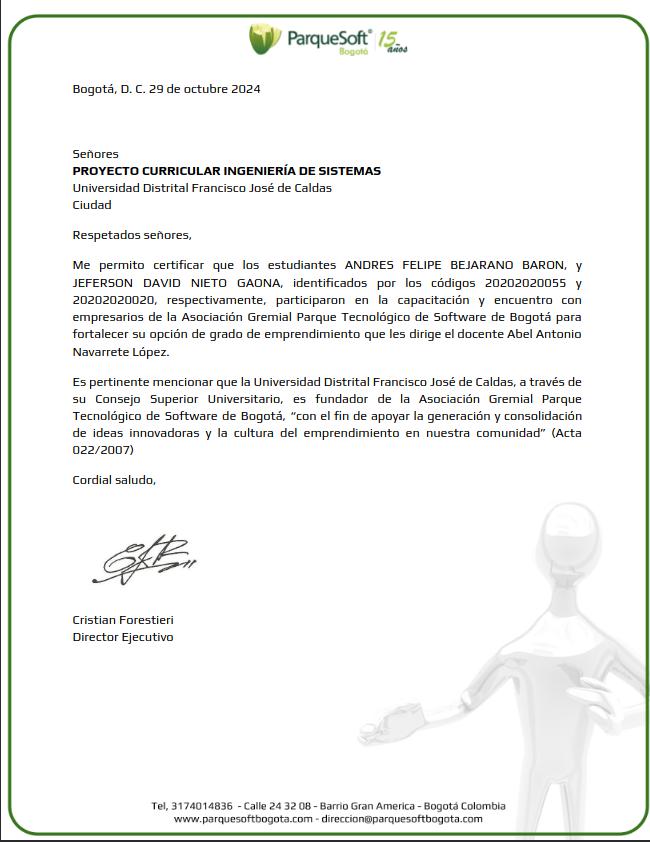
\includegraphics[width=0.7\textwidth]{Content/Images/CartaParquesoft.png}
        \footnote{Nota. \textup{Fuente: Autores }}
